%=====================================================================
%  Persistent Memory Architecture in Agents Using DBMS
%  Term Paper -- Thematic Assessment
%  Harshit Khemani (241302081)
%  B.Tech CSE (AI/ML), Section C
%  Department of Computer Science & Engineering, SGT University
%
%  Typography: XCharter (body) + Fira Sans (headings) + Inconsolata (code)
%  Measure held near 70 characters. Two hues only, plus cool neutrals.
%  Prose follows ASD-STE100: active voice, simple tense, short sentences.
%=====================================================================
\documentclass[11pt,a4paper]{article}

%---------------------------- fonts ---------------------------------
\usepackage[T1]{fontenc}
\usepackage[utf8]{inputenc}
\usepackage{XCharter}                    % body serif
\usepackage[scaled=0.95]{FiraSans}       % sans, for headings and labels
\usepackage[varqu,scaled=0.98]{zi4}      % Inconsolata mono
% Charter-matched math. Without it, the few symbols in the diagrams fall
% back to Computer Modern, which has no 26pt design size and warns.
\usepackage[charter,vvarbb]{newtxmath}
% FiraSans claims \familydefault on load. Hand it back to the serif so
% running text is XCharter and only \sffamily reaches for Fira.
\renewcommand{\familydefault}{\rmdefault}
\usepackage[letterspace=80]{microtype}

%---------------------------- layout --------------------------------
% Measure ~70 characters: 13.5cm of text on a 21cm page.
\usepackage[a4paper,top=2.8cm,bottom=2.8cm,left=3.75cm,right=3.75cm,
            headheight=14pt,footskip=1.1cm]{geometry}

\usepackage{graphicx}
\usepackage{booktabs}
\usepackage{tabularx}
\usepackage{array}
\usepackage[table,dvipsnames]{xcolor}
\usepackage{listings}
\usepackage{enumitem}
\usepackage{fancyhdr}
\usepackage{titlesec}
\usepackage{caption}
\usepackage{float}
\usepackage{tikz}
\usetikzlibrary{positioning,arrows.meta,fit,calc,shapes.geometric,
                decorations.pathreplacing}
\usepackage[hidelinks,breaklinks=true]{hyperref}
\usepackage{xurl}

\hypersetup{
  pdftitle={Persistent Memory Architecture in Agents Using DBMS},
  pdfauthor={Harshit Khemani (241302081)},
  pdfsubject={Database Management Systems --- Term Paper},
  pdfkeywords={agent memory, DBMS, sessions, schema, recall, SQLite, PostgreSQL}
}

%---------------------------- colour --------------------------------
% Two hues only. Blue carries structure, clay carries files and
% anything the agent does not own. Neutrals are cool so they agree
% with the blue. Every text colour clears 4.5:1 on white.
\definecolor{ink}     {HTML}{1A1D21}
\definecolor{blue800} {HTML}{1E3A5F}
\definecolor{blue600} {HTML}{35618F}
\definecolor{blue200} {HTML}{C2D5E8}
\definecolor{blue100} {HTML}{E8EFF7}
\definecolor{clay700} {HTML}{8A5A2B}
\definecolor{clay200} {HTML}{E6D3BC}
\definecolor{clay100} {HTML}{F7EEE3}
\definecolor{grey600} {HTML}{5C6570}
\definecolor{grey300} {HTML}{CBD0D7}
\definecolor{grey100} {HTML}{F1F3F6}

\color{ink}

%------------------------ vertical rhythm ---------------------------
% Body leading 1.45. Paragraphs separate by space, not indent.
\linespread{1.16}\selectfont
\setlength{\parindent}{0pt}
\setlength{\parskip}{0.62\baselineskip}
\setlist{topsep=0.3\baselineskip,itemsep=0.18\baselineskip,parsep=0pt,
         leftmargin=1.25em}

% Print hygiene: no orphans, no widows, no stretched pages.
\clubpenalty=10000
\widowpenalty=10000
\displaywidowpenalty=10000
\raggedbottom
\setlength{\emergencystretch}{1.5em}
\renewcommand{\arraystretch}{1.25}

%---------------------------- headers -------------------------------
\pagestyle{fancy}
\fancyhf{}
\fancyhead[L]{\footnotesize\sffamily\color{grey600}%
  Persistent Memory Architecture in Agents Using DBMS}
\fancyhead[R]{\footnotesize\sffamily\color{grey600}%
  \href{https://www.khe.money}{Harshit Khemani}}
\fancyfoot[C]{\footnotesize\sffamily\color{grey600}\thepage}
\renewcommand{\headrulewidth}{0.4pt}
\renewcommand{\headrule}{\color{grey300}%
  \hrule height 0.4pt width \headwidth}
\fancypagestyle{plain}{\fancyhf{}%
  \fancyfoot[C]{\footnotesize\sffamily\color{grey600}\thepage}%
  \renewcommand{\headrulewidth}{0pt}}

%---------------------------- headings ------------------------------
% Display type gets tight leading and slightly negative tracking.
\titleformat{\section}
  {\sffamily\bfseries\large\color{blue800}}{\thesection}{0.65em}{}
\titlespacing*{\section}{0pt}{1.5\baselineskip}{0.45\baselineskip}
\titleformat{\subsection}
  {\sffamily\bfseries\normalsize\color{ink}}{\thesubsection}{0.6em}{}
\titlespacing*{\subsection}{0pt}{1.05\baselineskip}{0.25\baselineskip}

%---------------------------- captions ------------------------------
\captionsetup{font={small},labelfont={sf,bf,color=blue800},
              labelsep=period,skip=7pt,width=0.95\textwidth}

%---------------------------- listings ------------------------------
\lstdefinestyle{base}{
  backgroundcolor=\color{grey100},
  basicstyle=\ttfamily\scriptsize\color{ink},
  keywordstyle=\color{blue800}\bfseries,
  stringstyle=\color{clay700},
  commentstyle=\color{grey600},   % Inconsolata ships no italic; colour alone marks comments
  numbers=none,
  showstringspaces=false,
  breaklines=true,
  frame=leftline,
  framerule=1.6pt,
  rulecolor=\color{blue200},
  framexleftmargin=6pt,
  xleftmargin=8pt,
  tabsize=2,
  captionpos=b,
  columns=fullflexible,
  keepspaces=true,
  aboveskip=0.7\baselineskip,
  belowskip=0.4\baselineskip
}
\lstset{style=base}
\lstdefinestyle{sql}{style=base,language=SQL,
  morekeywords={CONFLICT,GENERATED,ALWAYS,STORED,EXCLUDE,USING,GIST,HNSW,
    JSONB,TSVECTOR,VECTOR,tstzrange,SERIALIZABLE,OVER,SKIP,LOCKED,POLICY,
    RETURNING}}
\lstdefinelanguage{TypeScript}{
  keywords={const,let,export,default,async,await,return,if,function,new},
  sensitive=true, comment=[l]{//},
  morestring=[b]', morestring=[b]", morestring=[b]`}
\lstdefinestyle{ts}{style=base,language=TypeScript}

%---------------------------- helpers -------------------------------
\newcommand{\code}[1]{\texttt{\small #1}}
\newcommand{\tikzcode}[1]{\texttt{#1}}
\newcolumntype{L}[1]{>{\raggedright\arraybackslash}p{#1}}
\newcommand{\khe}{\href{https://www.khe.money}{Harshit Khemani}}
\newcommand{\aorg}{\href{https://agents.org.in}{AgentsORG}}
% Uppercase labels need loosened tracking.
\newcommand{\eyebrow}[1]{{\sffamily\footnotesize\bfseries\color{clay700}%
  \MakeUppercase{\textls[140]{#1}}}}

% ER entity: a name over a rule over its attributes.
\newcommand{\erE}[2]{\begin{tabular}{@{}l@{}}\textbf{#1}\\[1pt]\hline
  \\[-7pt]#2\end{tabular}}
\newcommand{\pk}[1]{\underline{#1}}
\newcommand{\fk}[1]{\textit{#1}}
\newcommand{\erlegend}{Underline marks a primary key. Italics mark a
  foreign key.}

%---------------------------- tikz ----------------------------------
% Monospace inside a diagram follows the node size, never \small.
\tikzset{every picture/.append style={
  execute at begin picture={\let\code\tikzcode\linespread{1.0}\selectfont}}}
\tikzset{
  box/.style   ={draw=blue200, line width=0.7pt, fill=blue100,
                 rounded corners=2pt, align=center, inner sep=5pt,
                 font=\sffamily\footnotesize},
  boxc/.style  ={draw=clay200, line width=0.7pt, fill=clay100,
                 rounded corners=2pt, align=center, inner sep=5pt,
                 font=\sffamily\footnotesize},
  boxn/.style  ={draw=grey300, line width=0.7pt, fill=white,
                 rounded corners=2pt, align=center, inner sep=5pt,
                 font=\sffamily\footnotesize},
  ent/.style   ={draw=blue200, line width=0.7pt, fill=blue100,
                 rounded corners=2pt, align=left, inner sep=4pt,
                 font=\sffamily\scriptsize},
  entc/.style  ={draw=clay200, line width=0.7pt, fill=clay100,
                 rounded corners=2pt, align=left, inner sep=4pt,
                 font=\sffamily\scriptsize},
  entn/.style  ={draw=grey300, line width=0.7pt, fill=white, dashed,
                 rounded corners=2pt, align=left, inner sep=4pt,
                 font=\sffamily\scriptsize},
  ar/.style    ={-{Stealth[length=2mm]}, draw=blue600, line width=0.7pt},
  arn/.style   ={-{Stealth[length=2mm]}, draw=grey300, line width=0.7pt,
                 dashed},
  tag/.style   ={font=\sffamily\scriptsize, text=grey600, inner sep=2pt},
  card/.style  ={font=\sffamily\scriptsize, text=grey600, fill=white,
                 inner sep=1.5pt},
  note/.style  ={font=\sffamily\scriptsize, text=clay700, align=left}
}

\begin{document}

%=====================================================================
%  TITLE PAGE
%=====================================================================
\begin{titlepage}
\centering
\sffamily
\linespread{1.0}\selectfont
\setlength{\parskip}{0pt}
\vspace*{1.2cm}

{\footnotesize\bfseries\color{grey600}%
 \textls[140]{SHREE GURU GOBIND SINGH TRICENTENARY UNIVERSITY}}\\[3pt]
{\footnotesize\color{grey600}Gurugram, Haryana}\\[1.1cm]

{\color{blue200}\rule{\textwidth}{1pt}}\\[9pt]
{\large\bfseries\color{ink}Department of Computer Science \& Engineering}\\[7pt]
{\color{blue200}\rule{\textwidth}{0.5pt}}\\[1.7cm]

\eyebrow{Term Paper \textperiodcentered\ Thematic Assessment}\\[9pt]
{\normalsize\color{grey600}Database Management Systems Laboratory}\\[1.4cm]

% A tabular with a \strut in every row: each row then has identical
% height and depth, so the two 7pt gaps render exactly equal. Plain \\
% breaks measure from the real glyph depth, and "Memory" (descender)
% would sit further from its neighbour than "Architecture in" (none).
{\fontsize{26}{30}\selectfont\bfseries\color{blue800}%
\begin{tabular}{@{}c@{}}
\strut Persistent Memory\\[7pt]
\strut Architecture in\\[7pt]
\strut Agents Using DBMS
\end{tabular}}\\[2.3cm]

\begin{minipage}{0.86\textwidth}
\small
\renewcommand{\arraystretch}{1.45}
\begin{tabular}{@{}r@{\hspace{1.5em}}l@{}}
{\color{grey600}Submitted by}  & \bfseries\khe \\
{\color{grey600}Roll number}   & 241302081 \\
{\color{grey600}Programme}     & B.Tech, Computer Science \& Engineering (AI/ML) \\
{\color{grey600}Section}       & C \\
{\color{grey600}Department}    & Computer Science \& Engineering \\
{\color{grey600}Institution}   & SGT University \\
\end{tabular}
\end{minipage}

\vfill
{\color{blue200}\rule{\textwidth}{0.5pt}}\\[6pt]
{\footnotesize\color{grey600}Academic Session 2026 \quad\textperiodcentered\quad
 Semester V}
\end{titlepage}

%=====================================================================
%  ABSTRACT
%=====================================================================
\pagenumbering{roman}
\setcounter{page}{2}

\section*{\sffamily\color{blue800}Abstract}
\addcontentsline{toc}{section}{Abstract}

A language model does not remember anything. It reads a prompt and it
writes a reply. After the reply, the model keeps nothing. An agent looks
like it remembers because a separate program saves its history and sends
that history back on the next call.

This paper studies that separate program. It shows that the program is a
database, and that the design of agent memory is ordinary database
design. The paper gives a four-layer architecture, a schema in
PostgreSQL, an index plan, a recall query, and the rules that keep two
agents from damaging each other's memory.

The paper then examines four real systems and asks one question of each:
\emph{how does this system remember something in session two that it
learned in session one?} \textbf{OpenClaw} keeps facts in Markdown files
and builds a SQLite index beside them. \textbf{Hermes Agent} keeps every
message in one SQLite file and limits its curated notes by a hard size
quota. \textbf{eve} saves the progress of the work itself, and
\textbf{Benji}, built on eve at \aorg, copies a lesson from one project
to all projects only after the lesson appears in three projects.
\textbf{Poke} keeps a separate log for each worker agent, and
\textbf{Code Storage} stores work as Git objects, where a merge settles
the conflict that a plain database can only reject.

\vspace{0.4\baselineskip}
\eyebrow{Keywords}\\[2pt]
agent memory, database management systems, sessions, schema design,
normalisation, indexing, recall, SQLite, PostgreSQL, Git.

\vspace{0.7\baselineskip}
{\setlength{\fboxsep}{9pt}%
\colorbox{clay100}{\parbox{\dimexpr\textwidth-18pt\relax}{\small
\eyebrow{A correction to two common claims}\\[3pt]
OpenAI did not buy OpenClaw. OpenAI hired the person who created it in
February 2026. The project moved to an independent foundation and it
kept the MIT licence \cite{tcOpenClaw,forbesOpenClaw}. Cognition bought
The Interaction Company, which makes Poke, in July 2026 \cite{tcPoke}.
No public record shows that anybody bought the Pierre Computer Company
\cite{pierreCo}. Section~\ref{sec:poke} marks clearly which statements
come from the documents and which statements are my own design.}}}

% Front-matter lists set their entries as paragraphs, so the document's
% \parskip would make them very airy. Suppress it inside them only.
\clearpage
{\sffamily\setlength{\parskip}{0pt}\tableofcontents}
\clearpage
{\sffamily\setlength{\parskip}{0pt}%
 \listoffigures
 \vspace{1.2\baselineskip}
 \listoftables}
\clearpage

\pagenumbering{arabic}
\setcounter{page}{1}

%=====================================================================
\section{Introduction}
%=====================================================================

\subsection{An agent forgets when a session ends}

A session is one continuous conversation between a user and an agent.
Inside a session the agent looks like it remembers. The program simply
resends the earlier text on every call.

The illusion breaks at the session boundary. The program starts the next
session with an empty prompt. Everything the agent learned on Monday is
gone on Thursday, unless some other component saved it.

\begin{figure}[H]
\centering
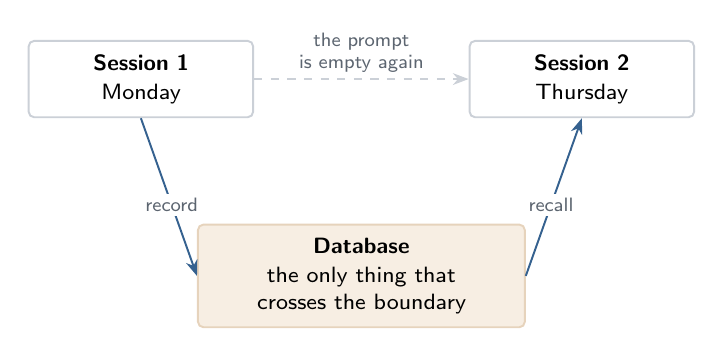
\begin{tikzpicture}
\node[boxn, text width=2.5cm] (s1) at (0,1.35)
  {\textbf{Session 1}\\[1pt]Monday};
\node[boxn, text width=2.5cm] (s2) at (5.6,1.35)
  {\textbf{Session 2}\\[1pt]Thursday};
\draw[arn] (s1) -- node[tag,above,align=center]
  {the prompt\\is empty again} (s2);
\node[boxc, text width=3.8cm] (db) at (2.8,-1.15)
  {\textbf{Database}\\[1pt]the only thing that\\crosses the boundary};
\draw[ar] (s1.south) -- node[card,pos=0.55]{record} (db.west);
\draw[ar] (db.east) -- node[card,pos=0.45]{recall} (s2.south);
\end{tikzpicture}
\caption[The session boundary]{Nothing survives a session boundary by itself. The agent must
record what it learns, and it must recall that material at the start of
the next session.}
\label{fig:gap}
\end{figure}

Two words carry a fixed meaning through this paper. To \textbf{record}
means to write something into the database. To \textbf{recall} means to
read something back out of it and put it into the prompt.

\subsection{Why a file is not enough}

Many agents start with a text file. A file works until the agent grows.
Then five problems appear, and every one of them is a problem that
databases already solve.

\begin{enumerate}
  \item One new fact touches several records. All of them must land, or
        none of them.
  \item The agent can stop in the middle of a task. It must not lose
        work that it already reported as finished.
  \item Two helper agents can write at the same time. A plain file loses
        one of the two writes.
  \item The agent must find facts by meaning and by exact word, and it
        must filter by date and by owner.
  \item Facts expire. A file keeps the old fact and the new fact side by
        side, and the agent then reads both.
\end{enumerate}

\subsection{Scope and method}

This paper covers how an agent keeps memory across sessions, and how a
database supports that. It does not cover model training, prompt design,
or agent planning.

I built the four case studies from public documents, public source
repositories, and reports. I cite each source where I use it. I ran no
experiments, so this paper reports no measurements of its own. Where a
company states a speed figure, I mark it as the company's claim.

%=====================================================================
\section{What the Agent Must Keep}
\label{sec:kinds}
%=====================================================================

An agent produces four kinds of material. Each kind has a different size,
a different read pattern, and a different cost when it is lost. One
storage design cannot serve all four well.

\begin{figure}[H]
\centering
\begin{tikzpicture}
\node[boxc, text width=5.3cm] (fact) at (0,1.05)
  {\textbf{Facts}\\[2pt]
   \scriptsize what is true: preferences, project rules\\
   \scriptsize small \textperiodcentered\ read on almost every turn};
\node[box, text width=5.3cm] (log) at (6.3,1.05)
  {\textbf{Session logs}\\[2pt]
   \scriptsize what happened: messages, tool results\\
   \scriptsize large \textperiodcentered\ searched only on demand};
\node[boxc, text width=5.3cm] (skill) at (0,-0.95)
  {\textbf{Skills}\\[2pt]
   \scriptsize how to act: saved procedures\\
   \scriptsize small \textperiodcentered\ chosen by name, not by meaning};
\node[box, text width=5.3cm] (art) at (6.3,-0.95)
  {\textbf{Work products}\\[2pt]
   \scriptsize what was made: code, documents\\
   \scriptsize versioned \textperiodcentered\ never overwritten};
\end{tikzpicture}
\caption[Four kinds of material]{The four kinds of material an agent must keep. The two on the
left stay small and the agent loads them often. The two on the right grow
without limit and the agent opens them only when it needs them.}
\label{fig:kinds}
\end{figure}

\begin{table}[H]
\centering
\caption[Material and its database structure]{How each kind of material maps onto database structures.}
\label{tab:kinds}
{\small
\begin{tabularx}{\textwidth}{L{2.1cm} X L{2.5cm}}
\toprule
\sffamily\bfseries Kind & \sffamily\bfseries Database structure &
\sffamily\bfseries Lifetime \\
\midrule
Facts & A small table of rows. Each row carries a subject, a statement,
a source, and a validity period. & Until a newer fact replaces it \\
Session logs & A large append-only table with a full-text index. &
Kept, then moved to cheap storage \\
Skills & A catalogue table with a name, tags, and a use count. &
Until somebody revises it \\
Work products & Content-addressed objects such as Git commits. &
Permanent and versioned \\
\bottomrule
\end{tabularx}}
\end{table}

The four kinds also differ in what a loss costs. If the agent loses a
session log, its recall gets weaker. If it loses a fact, its behaviour
changes. If it loses a work product, real work disappears. The system
should therefore protect the three kinds by different amounts.

%=====================================================================
\section{What a Database Gives the Agent}
%=====================================================================

Table~\ref{tab:req} lists what agent memory needs and names the database
mechanism that supplies it. The right column is the argument of this
paper in short form. Database systems already supply every item.

\begin{table}[H]
\centering
\caption[Requirements and mechanisms]{Requirements for agent memory, and the mechanism that meets each
one.}
\label{tab:req}
{\small
\begin{tabularx}{\textwidth}{L{3.5cm} X}
\toprule
\sffamily\bfseries Requirement & \sffamily\bfseries Mechanism \\
\midrule
Work must survive a crash & Write-ahead log and checkpoints \\
One fact writes several rows together & Transactions \\
Two agents write at once & Multiversion concurrency control \\
A recalled fact must point at a real message & Foreign keys \\
Search by meaning and by exact word & A vector index and a text index \\
Old facts must stop appearing & A validity period on every fact \\
An operator must see why the agent believes something & A link to the
source message \\
The prompt must stay small & A strict limit on how many rows recall
returns \\
One system serves many users & A tenant column and row-level security \\
\bottomrule
\end{tabularx}}
\end{table}

Two of these rows deserve a note.

The prompt limit is the hardest constraint. A normal database tries to
read as few disk pages as possible. Here the scarce resource is the
prompt. A recall that returns fifty correct rows has failed if six rows
were enough. The memory layer must therefore throw away most of what it
finds.

The validity period is the row that deployed systems most often skip.
Without it the agent recalls a fact and its replacement at the same time.
Section~\ref{sec:validity} shows the repair.

%=====================================================================
\section{The Architecture}
\label{sec:arch}
%=====================================================================

I separate the design into four layers. Each layer holds a different kind
of material and offers a different guarantee.

\begin{figure}[H]
\centering
\begin{tikzpicture}[
  lay/.style={draw=blue200, line width=0.7pt, fill=blue100,
              rounded corners=2pt, minimum height=1.02cm,
              text width=8.3cm, align=center, inner sep=4pt,
              font=\sffamily\footnotesize}]
\node[lay, fill=clay100, draw=clay200] (l4)
  {\textbf{Layer 4 \textperiodcentered\ The prompt}\\[1pt]
   \scriptsize what the model sees right now \textperiodcentered\ nothing is saved here};
\node[lay, below=0.42cm of l4] (l3)
  {\textbf{Layer 3 \textperiodcentered\ Indexes}\\[1pt]
   \scriptsize a vector index and a text index \textperiodcentered\ rebuildable};
\node[lay, below=0.42cm of l3] (l2)
  {\textbf{Layer 2 \textperiodcentered\ Tables}\\[1pt]
   \scriptsize sessions, messages, facts, skills \textperiodcentered\ this layer holds the constraints};
\node[lay, below=0.42cm of l2] (l1)
  {\textbf{Layer 1 \textperiodcentered\ The log}\\[1pt]
   \scriptsize every message and every action, in order, never changed};

\draw[ar] (l1) -- node[tag,right=2pt]{derive} (l2);
\draw[ar] (l2) -- node[tag,right=2pt]{index} (l3);
\draw[ar] (l3) -- node[tag,right=2pt]{recall} (l4);
\draw[ar] ($(l4.west)+(-0.2,0)$) to[out=180,in=180,looseness=1.1]
  node[tag,left=2pt,align=right]{record} ($(l1.west)+(-0.2,0)$);
\end{tikzpicture}
\caption[The four layers]{The four layers. Layer 1 is the only original copy. The system
can rebuild layers 2 and 3 from it. Layer 4 disappears after every model
call.}
\label{fig:layers}
\end{figure}

\textbf{Layer 1 holds the log.} The agent appends every message, every
tool call, and every result. It never edits a row here. This layer buys
three things. The team can drop layers 2 and 3 and build them again when
the embedding model changes. An operator can replay the log and see why
the agent acted. A crashed agent can restart from the last entry.

\textbf{Layer 2 holds the tables.} This layer stores sessions, messages,
facts, and skills. Constraints live here, so this is the layer that makes
promises. Section~\ref{sec:schema} gives the schema.

\textbf{Layer 3 holds the indexes.} An index is derived data. It can fall
behind the table, and the team can always build it again.

\textbf{Layer 4 is the prompt.} It is small, expensive, and temporary.
Every other layer exists to keep it short and correct.

\subsection{How the agent records a fact}

Recording is not one \code{INSERT}. The agent runs five steps, and the
first four must succeed together or fail together.

\begin{figure}[H]
\centering
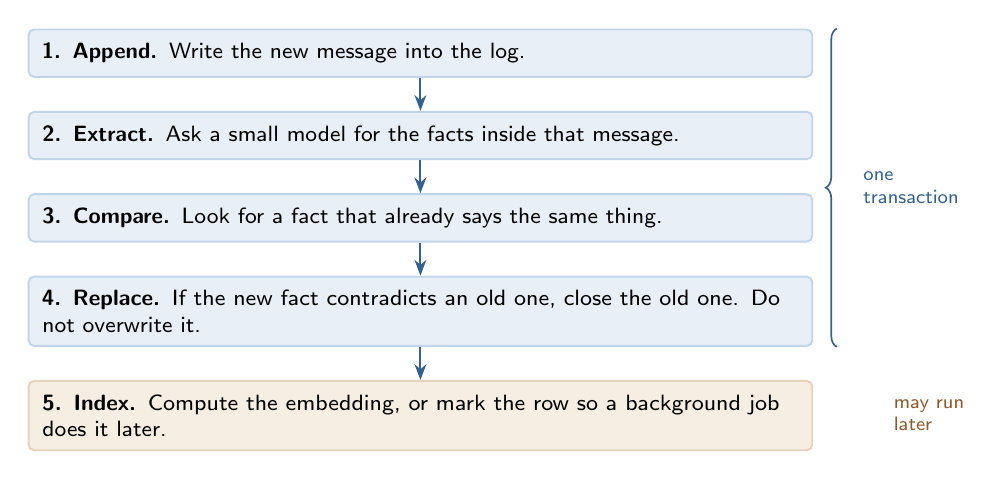
\begin{tikzpicture}[node distance=0.42cm,
  st/.style={draw=blue200, line width=0.7pt, fill=blue100,
             rounded corners=2pt, text width=9.6cm, align=left,
             inner sep=5pt, font=\sffamily\footnotesize}]
\node[st] (a) {\textbf{1. Append.} Write the new message into the log.};
\node[st, below=of a] (b) {\textbf{2. Extract.} Ask a small model for the
  facts inside that message.};
\node[st, below=of b] (c) {\textbf{3. Compare.} Look for a fact that
  already says the same thing.};
\node[st, below=of c] (d) {\textbf{4. Replace.} If the new fact
  contradicts an old one, close the old one. Do not overwrite it.};
\node[st, below=of d, fill=clay100, draw=clay200] (e)
  {\textbf{5. Index.} Compute the embedding, or mark the row so a
   background job does it later.};

\foreach \x/\y in {a/b,b/c,c/d,d/e} \draw[ar] (\x) -- (\y);

\draw[decorate, decoration={brace,amplitude=4pt,mirror},
      draw=blue600, line width=0.6pt]
  ($(a.north east)+(3mm,0)$) -- ($(d.south east)+(3mm,0)$)
  node[midway, right=6pt, font=\sffamily\scriptsize, text=blue600,
       align=left] {one\\transaction};
\node[note, right=9mm of e] {may run\\later};
\end{tikzpicture}
\caption[The record path]{The record path. Step 5 can run later, which is exactly why the
schema carries a flag that marks an index entry as out of date.}
\label{fig:record}
\end{figure}

\subsection{How the agent recalls a fact}

At the start of a session the agent asks the database for a small set of
rows. Two searches run, and the system merges their results.

\begin{figure}[H]
\centering
\resizebox{\textwidth}{!}{%
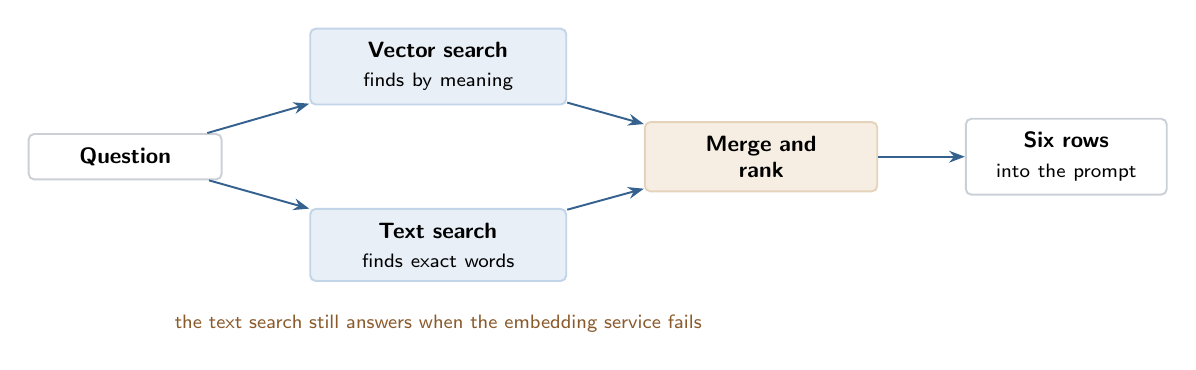
\begin{tikzpicture}[node distance=0.55cm]
\node[boxn, text width=2.1cm] (q) {\textbf{Question}};
\node[box, above right=0.35cm and 1.1cm of q, text width=2.9cm] (v)
  {\textbf{Vector search}\\[1pt]\scriptsize finds by meaning};
\node[box, below right=0.35cm and 1.1cm of q, text width=2.9cm] (t)
  {\textbf{Text search}\\[1pt]\scriptsize finds exact words};
\node[boxc, right=5.35cm of q, text width=2.6cm] (m)
  {\textbf{Merge and\\rank}};
\node[boxn, right=1.1cm of m, text width=2.2cm] (k)
  {\textbf{Six rows}\\[1pt]\scriptsize into the prompt};

\draw[ar] (q) -- (v);
\draw[ar] (q) -- (t);
\draw[ar] (v) -- (m);
\draw[ar] (t) -- (m);
\draw[ar] (m) -- (k);
\node[note, below=0.3cm of t, align=center]
  {the text search still answers when the embedding service fails};
\end{tikzpicture}}
\caption[The recall path]{The recall path. Vector search alone misses file names, error
strings, and version numbers, so every system in this paper runs a text
search beside it.}
\label{fig:recall}
\end{figure}

The system ranks the merged rows by three signals. It prefers a row that
both searches found. It prefers a row that the user marked as important.
It prefers a recent row, unless somebody marked the row as permanent.
OpenClaw halves the weight of a dated note every thirty days and never
reduces the weight of a curated note \cite{openclawMemCfg}.

\subsection{How the agent forgets}

Three different operations hide behind the word \emph{forget}. Keep them
separate.

\begin{itemize}
  \item \textbf{Rank lower.} The row stays. Recall stops returning it.
  \item \textbf{Move.} The row goes to cheap storage. The agent can still
        read it, but more slowly.
  \item \textbf{Delete.} The row goes away for good. This is a legal
        action, not a speed improvement, and the team must also redact
        the log entry.
\end{itemize}

A fourth method works better than all three for curated notes. Hermes
Agent sets a hard size limit and returns an \emph{error} when a write
would pass it \cite{hermesMemory}. The agent must then merge or drop a
note before it can add one. A quota is easier to reason about than a
background cleanup job.

%=====================================================================
\section{The Schema}
\label{sec:schema}
%=====================================================================

\begin{figure}[H]
\centering
\resizebox{\textwidth}{!}{%
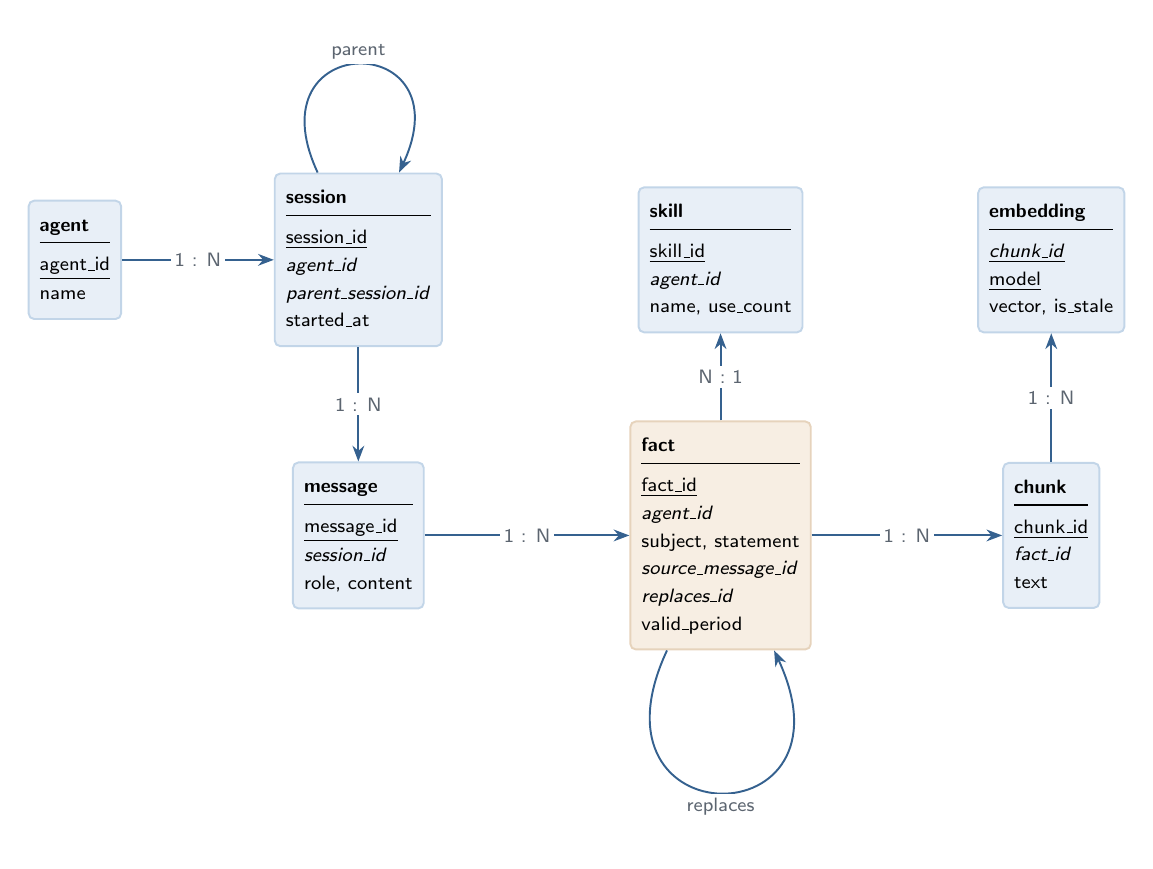
\begin{tikzpicture}
% Two rows, left to right, so no relationship line crosses another.
\node[ent]  (agent) at (0,3.5)   {\erE{agent}{\pk{agent\_id}\\ name}};
\node[ent]  (sess)  at (3.6,3.5)
  {\erE{session}{\pk{session\_id}\\ \fk{agent\_id}\\ \fk{parent\_session\_id}\\ started\_at}};
\node[ent]  (skill) at (8.2,3.5)
  {\erE{skill}{\pk{skill\_id}\\ \fk{agent\_id}\\ name, use\_count}};
\node[ent]  (emb)   at (12.4,3.5)
  {\erE{embedding}{\pk{\fk{chunk\_id}}\\ \pk{model}\\ vector, is\_stale}};
\node[ent]  (msg)   at (3.6,0.0)
  {\erE{message}{\pk{message\_id}\\ \fk{session\_id}\\ role, content}};
\node[entc] (fact)  at (8.2,0.0)
  {\erE{fact}{\pk{fact\_id}\\ \fk{agent\_id}\\ subject, statement\\
    \fk{source\_message\_id}\\ \fk{replaces\_id}\\ valid\_period}};
\node[ent]  (chunk) at (12.4,0.0)
  {\erE{chunk}{\pk{chunk\_id}\\ \fk{fact\_id}\\ text}};

\draw[ar] (agent) -- node[card,pos=0.5]{1 : N} (sess);
\draw[ar] (sess)  -- node[card,pos=0.5]{1 : N} (msg);
\draw[ar] (msg)   -- node[card,pos=0.5]{1 : N} (fact);
\draw[ar] (fact)  -- node[card,pos=0.5]{1 : N} (chunk);
\draw[ar] (chunk) -- node[card,pos=0.5]{1 : N} (emb);
\draw[ar] (fact)  -- node[card,pos=0.5]{N : 1} (skill);
% A short loop on one side reads as a self-relationship. An arc drawn
% between two corners of the same node reads as a stray triangle.
\path (sess) edge[ar, loop above, looseness=5, min distance=7mm,
                  out=115, in=65] node[card, above]{parent} (sess);
\path (fact) edge[ar, loop below, looseness=5, min distance=7mm,
                  out=245, in=295] node[card, below]{replaces} (fact);
\end{tikzpicture}}
\caption[The schema]{The schema. Two relationships point back at their own table.
\code{parent\_session\_id} keeps the link when the agent shortens a long
session, and \code{replaces\_id} lets a new fact retire an old one
without erasing it. \erlegend}
\label{fig:er}
\end{figure}

\subsection{The tables}

\begin{lstlisting}[style=sql,caption={The core tables in PostgreSQL.}]
CREATE TABLE session (
    session_id        uuid PRIMARY KEY,
    agent_id          uuid NOT NULL REFERENCES agent ON DELETE CASCADE,
    -- when the agent shortens a session, the short one points here
    parent_session_id uuid REFERENCES session(session_id),
    channel           text NOT NULL
                        CHECK (channel IN ('cli','web','chat','api')),
    started_at        timestamptz NOT NULL DEFAULT now()
);

CREATE TABLE message (
    message_id  bigserial PRIMARY KEY,
    session_id  uuid NOT NULL REFERENCES session ON DELETE CASCADE,
    seq         integer NOT NULL,
    role        text NOT NULL
                  CHECK (role IN ('user','assistant','tool')),
    content     text NOT NULL,
    content_tsv tsvector GENERATED ALWAYS AS
                  (to_tsvector('english', content)) STORED,
    UNIQUE (session_id, seq)
);

CREATE TABLE fact (
    fact_id           bigserial PRIMARY KEY,
    agent_id          uuid NOT NULL REFERENCES agent ON DELETE CASCADE,
    subject           text NOT NULL,
    statement         text NOT NULL,
    is_permanent      boolean NOT NULL DEFAULT false,
    -- why does the agent believe this?
    source_message_id bigint REFERENCES message ON DELETE SET NULL,
    replaces_id       bigint REFERENCES fact(fact_id),
    -- the period during which this fact is true
    valid_period      tstzrange NOT NULL DEFAULT tstzrange(now(), NULL),
    last_used_at      timestamptz NOT NULL DEFAULT now(),
    -- the agent holds ONE live fact per subject at any moment
    EXCLUDE USING gist (agent_id WITH =, subject WITH =,
                        valid_period WITH &&)
);

CREATE TABLE embedding (
    chunk_id  bigint NOT NULL REFERENCES chunk ON DELETE CASCADE,
    model     text NOT NULL,
    vector    vector(1536) NOT NULL,
    is_stale  boolean NOT NULL DEFAULT false,
    PRIMARY KEY (chunk_id, model)
);
\end{lstlisting}

\subsection{Normalisation}

A first version of an agent usually writes one wide table. It stores the
session, the agent name, the model name, the message, the extracted fact,
and the skill name in a single row. That table repeats the agent name on
every row, and it repeats the model name with it. Table~\ref{tab:norm}
shows what breaks.

\begin{table}[H]
\centering
\caption[Faults in one wide table]{Three faults in the single wide table, and what each one costs.}
\label{tab:norm}
{\small
\begin{tabularx}{\textwidth}{L{2.4cm} X}
\toprule
\sffamily\bfseries Fault & \sffamily\bfseries What happens \\
\midrule
Update fault & An operator changes the agent's model. The database must
rewrite every historical row. \\
Insert fault & A session starts with no messages yet. The table cannot
record the session at all. \\
Delete fault & Somebody deletes the last message of a session. The fact
that the session existed disappears with it. \\
\bottomrule
\end{tabularx}}
\end{table}

The repair splits the wide table into \code{agent}, \code{session},
\code{message}, \code{fact}, \code{chunk}, \code{embedding}, and
\code{skill}. Each table then has one key, and every column describes
that key and nothing else. The schema reaches Boyce--Codd normal form.
Every join follows a foreign key, so the split loses no information.

I break the rule in three places on purpose:

\begin{itemize}
  \item \code{tool\_calls} stays as one JSON column. Its shape changes
        with every model provider, so a fixed set of columns would be
        wrong within a year.
  \item \code{agent\_id} repeats on child tables. A security rule then
        reads it without a join, and that rule runs on every query.
  \item \code{content\_tsv} repeats the text in searchable form. This
        buys the text index, and it is the same trade any index makes.
\end{itemize}

\subsection{Indexes}

\begin{table}[H]
\centering
\caption[Indexes by question]{One index for each kind of question the agent asks.}
\label{tab:index}
{\small
\begin{tabularx}{\textwidth}{L{3.0cm} L{2.6cm} X}
\toprule
\sffamily\bfseries Question & \sffamily\bfseries Index &
\sffamily\bfseries Reason \\
\midrule
``What is similar?'' & HNSW on the vector & Finds near vectors without
reading them all \\
``Which row has this word?'' & GIN on the text & Finds names and error
strings that vectors miss \\
``Which rows are live now?'' & GiST on the period & Also enforces the
one-live-fact rule \\
``Which rows belong to this agent?'' & Partial B-tree & Keeps retired
rows off the fast path \\
\bottomrule
\end{tabularx}}
\end{table}

\begin{lstlisting}[style=sql,caption={The indexes.}]
CREATE INDEX ix_emb_vec  ON embedding USING hnsw (vector vector_cosine_ops);
CREATE INDEX ix_fact_tsv ON fact USING gin  (to_tsvector('english', statement));
CREATE INDEX ix_fact_per ON fact USING gist (valid_period);

-- Recall only ever reads facts that are still true.
CREATE INDEX ix_fact_live ON fact (agent_id, last_used_at DESC)
    WHERE upper_inf(valid_period);
\end{lstlisting}

\subsection{The recall query}

\begin{lstlisting}[style=sql,caption={Recall. The two searches run, the results merge, and the query returns six rows.}]
WITH live AS (
    -- Apply the owner filter and the date filter one time only.
    SELECT f.fact_id, f.statement, f.is_permanent, f.last_used_at
    FROM   fact f
    WHERE  f.agent_id = $1
      AND  f.valid_period @> now()
),
by_meaning AS (
    SELECT l.fact_id,
           ROW_NUMBER() OVER (ORDER BY MIN(e.vector <=> $2)) AS place
    FROM   live l
      JOIN chunk     c ON c.fact_id  = l.fact_id
      JOIN embedding e ON e.chunk_id = c.chunk_id AND NOT e.is_stale
    GROUP BY l.fact_id
    LIMIT 200
),
by_word AS (
    SELECT l.fact_id,
           ROW_NUMBER() OVER (
             ORDER BY ts_rank_cd(to_tsvector('english', l.statement),
                                 websearch_to_tsquery('english', $3)) DESC
           ) AS place
    FROM   live l
    WHERE  to_tsvector('english', l.statement)
             @@ websearch_to_tsquery('english', $3)
    LIMIT 200
)
SELECT l.fact_id, l.statement
FROM   live l
  LEFT JOIN by_meaning m ON m.fact_id = l.fact_id
  LEFT JOIN by_word    w ON w.fact_id = l.fact_id
WHERE  m.place IS NOT NULL OR w.place IS NOT NULL
ORDER  BY COALESCE(m.place, 999) + COALESCE(w.place, 999),
          l.is_permanent DESC,
          l.last_used_at DESC
LIMIT  6;    -- six rows, because the prompt is the scarce resource
\end{lstlisting}

\subsection{Old facts must not come back}
\label{sec:validity}

Every fact carries a period. When the agent learns something that
contradicts an old fact, it closes the old period and opens a new one. It
does not delete the old row.

\begin{figure}[H]
\centering
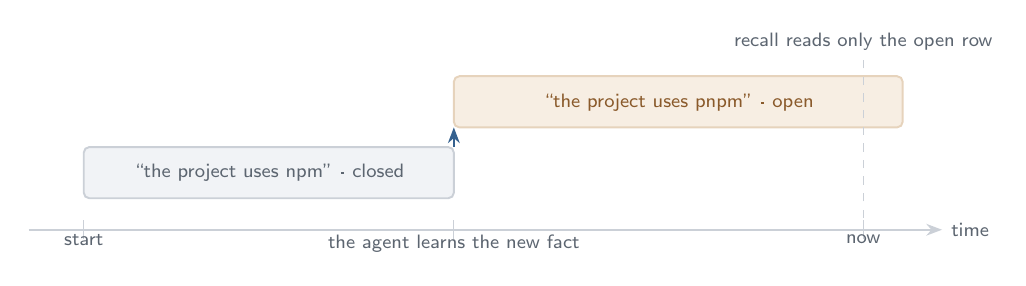
\begin{tikzpicture}
\draw[draw=grey300, line width=0.7pt, -{Stealth[length=2mm]}]
  (0,0) -- (11.6,0) node[tag, right=1pt] {time};
\foreach \x/\t in {0.7/{start}, 5.4/{the agent learns the new fact},
                   10.6/{now}}
  \draw[grey300] (\x,-0.12) -- (\x,0.12)
    node[tag, below=3pt, align=center, font=\sffamily\scriptsize] {\t};

\draw[fill=grey100, draw=grey300, rounded corners=2pt, line width=0.7pt]
  (0.7,0.4) rectangle (5.4,1.05);
\node[font=\sffamily\scriptsize, text=grey600] at (3.05,0.72)
  {``the project uses npm'' \textperiodcentered\ closed};

\draw[fill=clay100, draw=clay200, rounded corners=2pt, line width=0.7pt]
  (5.4,1.3) rectangle (11.1,1.95);
\node[font=\sffamily\scriptsize, text=clay700] at (8.25,1.62)
  {``the project uses pnpm'' \textperiodcentered\ open};

\draw[ar] (5.4,1.05) -- (5.4,1.3);
\draw[grey300, dashed] (10.6,0.15) -- (10.6,2.25);
\node[tag, above] at (10.6,2.2) {recall reads only the open row};
\end{tikzpicture}
\caption[A new fact retires an old one]{A new fact retires an old one. The old row stays for the audit
trail, but recall never returns it again.}
\label{fig:validity}
\end{figure}

This design also answers a question that a plain table cannot answer:
\emph{what did the agent believe last month?} An operator changes one
parameter in the query and reads the state at any past date.

%=====================================================================
\section{Two Agents That Write at the Same Time}
\label{sec:concurrent}
%=====================================================================

Modern agents start helper agents. When two helpers write to the same
memory, the system meets the classic problems of any multi-user database.
Table~\ref{tab:conc} lists the three that matter here.

\begin{table}[H]
\centering
\caption[Faults with two writers]{Three faults that appear when two agents write together.}
\label{tab:conc}
{\small
\begin{tabularx}{\textwidth}{L{3.2cm} X L{3.0cm}}
\toprule
\sffamily\bfseries Fault & \sffamily\bfseries What happens &
\sffamily\bfseries Repair \\
\midrule
A write disappears & Both helpers read the notes file, both add a line,
and the second write replaces the first. & Write single rows, not whole
files \\
A fact appears twice & Both helpers look for a fact, both find nothing,
and both insert it. & The \code{EXCLUDE} rule in the schema \\
An action repeats & The agent sends an email, then crashes before it
saves its progress. On restart it sends the email again. & A table of
completed actions \\
\bottomrule
\end{tabularx}}
\end{table}

The second fault is the one teams miss. The two helpers write
\emph{different} rows, so the database sees no conflict between them.
Each helper simply read a set that the other helper then changed. A
common isolation setting allows this. The schema in
Section~\ref{sec:schema} closes it, because the \code{EXCLUDE} rule makes
two live facts about one subject impossible to store. A rule in the
schema holds whatever the isolation setting is.

The third fault needs one small table. The agent records the action and
performs it inside the same transaction.

\begin{lstlisting}[style=sql,caption={A table of completed actions stops a repeat after a crash.}]
INSERT INTO completed_action (action_key, session_id, kind)
VALUES ($1, $2, 'send_email')
ON CONFLICT (action_key) DO NOTHING
RETURNING action_key;   -- no row means the agent already did it
\end{lstlisting}

%=====================================================================
\section{How Four Systems Remember}
%=====================================================================

This section asks one question of four real systems. \emph{How does the
system remember in session two what it learned in session one?}

\subsection{OpenClaw}
\label{sec:openclaw}

OpenClaw is an open assistant that runs on the user's own machine. A
local gateway manages its sessions, its channels, and its tools
\cite{openclawRepo}.

\textbf{How it remembers.} OpenClaw writes its long-term facts into
Markdown files. \code{MEMORY.md} holds facts about the user.
\code{USER.md} holds the user's profile. A dated file under
\code{memory/} holds each day's notes. The system then reads those files,
splits them into pieces, and stores the pieces with their vectors in a
SQLite database \cite{openclawMemCfg}. At the start of a new session the
agent searches that database and loads at most six pieces back into the
prompt.

\begin{figure}[H]
\centering
\resizebox{\textwidth}{!}{%
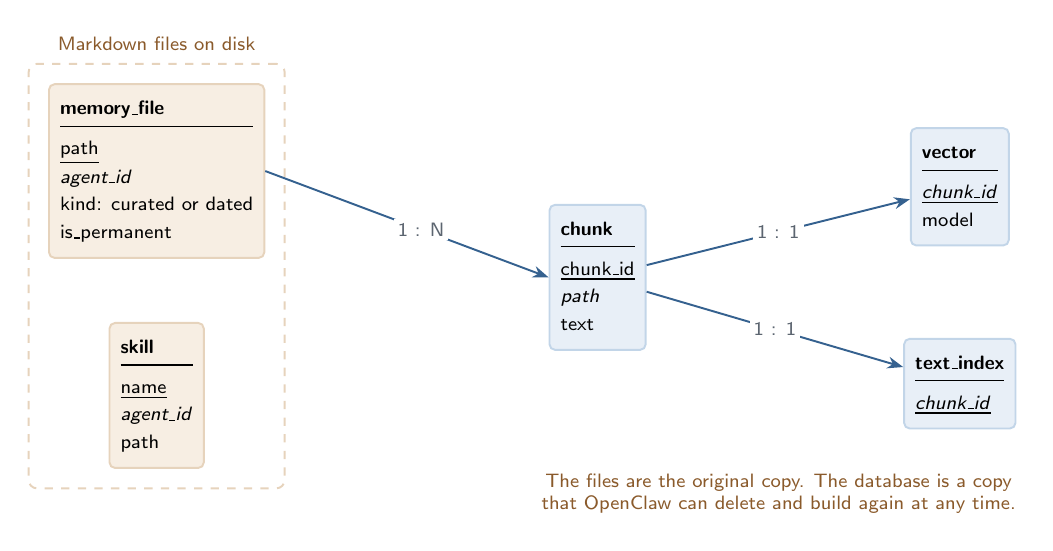
\begin{tikzpicture}
\node[entc] (files) at (0,1.35)
  {\erE{memory\_file}{\pk{path}\\ \fk{agent\_id}\\ kind: curated or dated\\ is\_permanent}};
\node[entc] (skill) at (0,-1.5)
  {\erE{skill}{\pk{name}\\ \fk{agent\_id}\\ path}};
% A dashed group says why skill has no relationship line: it is another
% file on disk, not a row that the index derives from.
\node[draw=clay200, line width=0.7pt, dashed, rounded corners=3pt,
      inner sep=7pt, fit=(files)(skill)] (disk) {};
\node[note, above=1pt of disk] {Markdown files on disk};

\node[ent] (chunk) at (5.6,0.0)
  {\erE{chunk}{\pk{chunk\_id}\\ \fk{path}\\ text}};
\node[ent] (vec) at (10.2,1.15)
  {\erE{vector}{\pk{\fk{chunk\_id}}\\ model}};
\node[ent] (fts) at (10.2,-1.35)
  {\erE{text\_index}{\pk{\fk{chunk\_id}}}};

\draw[ar] (files.east) -- node[card,pos=0.55]{1 : N} (chunk.west);
\draw[ar] (chunk) -- node[card,pos=0.5]{1 : 1} (vec);
\draw[ar] (chunk) -- node[card,pos=0.5]{1 : 1} (fts);

\node[note, align=center] at (7.9,-2.75)
  {The files are the original copy. The database is a copy\\
   that OpenClaw can delete and build again at any time.};
\end{tikzpicture}}
\caption[OpenClaw]{OpenClaw. Clay boxes are Markdown files and blue boxes are
SQLite tables. \erlegend}
\label{fig:er-openclaw}
\end{figure}

\textbf{What this design buys.} The files stay readable, so a person can
open them and correct a wrong fact. The database is a copy, so OpenClaw
can delete it and build it again when the embedding model changes. The
documents state that the team must run a rebuild command after such a
change \cite{openclawMemCfg}. Text search also acts as the safety net.
When the embedding service fails, OpenClaw still answers from the text
index alone.

\textbf{What it costs.} OpenClaw keeps one database file for each agent.
A query that spans two agents therefore cannot use a join. The program
must read both files and merge the results itself.

\textbf{One note on the project.} OpenAI hired the creator of OpenClaw in
February 2026. OpenAI did not buy the project. The project moved to an
independent foundation and it kept the MIT licence
\cite{tcOpenClaw,forbesOpenClaw}.

\subsection{Hermes Agent}
\label{sec:hermes}

Hermes Agent comes from Nous Research. It runs from a terminal, from a
chat gateway, and from a code editor, and all three paths use one agent
class \cite{hermesArch}.

\textbf{How it remembers.} Hermes splits memory in two. Every message
from every session goes into one SQLite file. A full-text index sits over
those messages, so the agent can search months of history and read the
real sentences back \cite{hermesMemory}. Beside that file sit two small
Markdown notes. \code{MEMORY.md} holds about 800 tokens and
\code{USER.md} holds about 500 tokens. Hermes loads both notes at the
start of a session and fixes them into the prompt.

\begin{figure}[H]
\centering
\resizebox{\textwidth}{!}{%
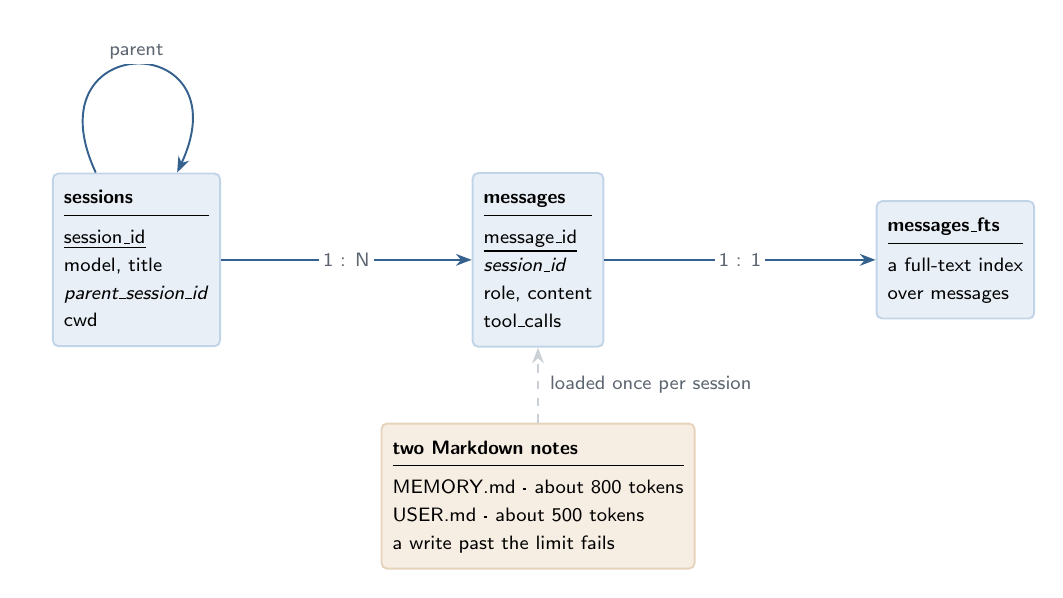
\begin{tikzpicture}
\node[ent] (sess) at (0,1.5)
  {\erE{sessions}{\pk{session\_id}\\ model, title\\ \fk{parent\_session\_id}\\ cwd}};
\node[ent] (msg) at (5.1,1.5)
  {\erE{messages}{\pk{message\_id}\\ \fk{session\_id}\\ role, content\\ tool\_calls}};
\node[ent] (fts) at (10.4,1.5)
  {\erE{messages\_fts}{\scriptsize a full-text index\\ \scriptsize over messages}};
\node[entc] (files) at (5.1,-1.5)
  {\erE{two Markdown notes}{MEMORY.md \textperiodcentered\ about 800 tokens\\
    USER.md \textperiodcentered\ about 500 tokens\\
    a write past the limit fails}};

\draw[ar] (sess) -- node[card,pos=0.5]{1 : N} (msg);
\draw[ar] (msg)  -- node[card,pos=0.5]{1 : 1} (fts);
\path (sess) edge[ar, loop above, looseness=5, min distance=7mm,
                  out=115, in=65] node[card, above]{parent} (sess);
\draw[arn] (files) -- node[tag,right=2pt]{loaded once per session} (msg);
\end{tikzpicture}}
\caption[Hermes Agent]{Hermes Agent. One SQLite file holds unlimited history. Two small
files hold the notes, and those notes have a hard size limit.
\erlegend}
\label{fig:er-hermes}
\end{figure}

\textbf{Three decisions worth copying.} First, the notes have a hard
limit and a write past that limit returns an error \cite{hermesMemory}.
The agent must therefore merge two notes before it writes a third. A
quota beats a cleanup job, because the agent sees the quota and can act
on it. Second, a session that grows too long becomes a shorter child
session, and \code{parent\_session\_id} keeps the link
\cite{hermesDeepwiki}. Shortening a session therefore adds a row instead
of destroying one. Third, Hermes opens the database in write-ahead
logging mode so readers do not block the writer, and it falls back to a
simpler mode on network drives that cannot support it
\cite{hermesDeepwiki,sqliteWal}.

\textbf{The trade.} Hermes fixes the notes into the prompt at session
start. A note that the agent writes during a session does not appear
until the next session \cite{hermesMemory}. Hermes accepts a stale read
in exchange for a cheaper prompt.

\subsection{eve and Benji}
\label{sec:eve}

eve is Vercel's framework for agents that survive a restart. An agent is
a folder \cite{eveSite}. Benji is a design-review agent that \aorg\
builds on eve \cite{benjiRepo,agentsorg}.

\textbf{How eve remembers.} eve saves the progress of the work, not the
meaning of it. It splits work into sessions, turns, and steps, and it
writes a checkpoint at every step boundary \cite{eveDurability}. When the
process restarts, it continues from the last finished step instead of
repeating the whole turn. A durable store holds this state, and the team
chooses that store. On a server it can be PostgreSQL.

\begin{lstlisting}[style=ts,caption={Choosing PostgreSQL as the durable store in eve \cite{eveDurability}.}]
export default defineAgent({
  model: "anthropic/claude-opus-4.8",
  experimental: { workflow: { world: "@workflow/world-postgres" } },
});
\end{lstlisting}

eve also offers a named slot of durable state for one session. The
documents are strict about its limit. The slot belongs to one session, a
helper agent never shares it, and anything that must outlive the session
belongs in a separate database \cite{eveState}. That limit is the reason
two helper agents under eve cannot damage each other's memory. They hold
no shared cell.

\textbf{How Benji remembers.} Benji keeps two levels. The first level
holds notes about one repository, such as a person's stated preference.
The second level holds portable lessons. A note becomes a lesson only
after it appears in three separate repositories \cite{benjiRepo}.

\begin{figure}[H]
\centering
\resizebox{\textwidth}{!}{%
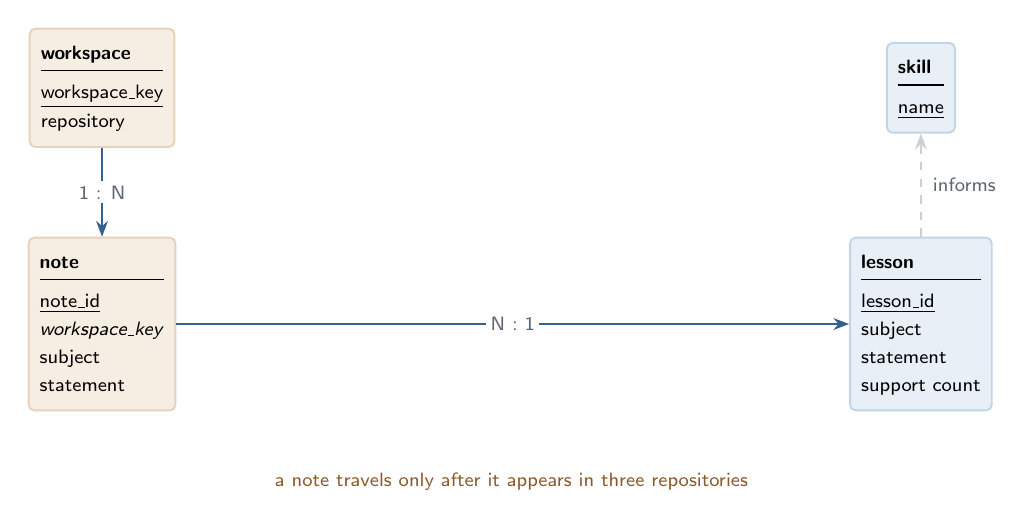
\begin{tikzpicture}
\node[entc] (ws) at (0,1.7) {\erE{workspace}{\pk{workspace\_key}\\ repository}};
\node[entc] (obs) at (0,-1.3)
  {\erE{note}{\pk{note\_id}\\ \fk{workspace\_key}\\ subject\\ statement}};
\node[ent] (les) at (10.4,-1.3)
  {\erE{lesson}{\pk{lesson\_id}\\ subject\\ statement\\ support count}};
\node[ent] (sk) at (10.4,1.7) {\erE{skill}{\pk{name}}};

\draw[ar] (ws) -- node[card,pos=0.5]{1 : N} (obs);
\draw[ar] (obs) -- node[card,pos=0.5]{N : 1} (les);
\draw[arn] (les) -- node[tag,right=2pt]{informs} (sk);
% Clear of the entity boxes, which reach down to about y = -2.5.
\node[note, align=center] at (5.2,-3.3)
  {a note travels only after it appears in three repositories};
\end{tikzpicture}}
\caption[Benji]{Benji. The rule that copies a note into a lesson is a count with
a threshold, and one SQL statement expresses it. \erlegend}
\label{fig:er-benji}
\end{figure}

The rule stops one project's habit from becoming a rule for every
project. It is a counting rule, and SQL states counting rules directly.

\begin{lstlisting}[style=sql,caption={Benji's promotion rule. The last line is the whole policy.}]
INSERT INTO lesson (agent_id, subject, statement, support_count)
SELECT n.agent_id, n.subject,
       (ARRAY_AGG(n.statement ORDER BY n.last_used_at DESC))[1],
       COUNT(DISTINCT n.workspace_key)
FROM   note n
GROUP  BY n.agent_id, n.subject
HAVING COUNT(DISTINCT n.workspace_key) >= 3;
\end{lstlisting}

\textbf{Where Benji stands today.} Benji stores both levels in JSON files
\cite{benjiRepo}. That choice keeps the data readable, and it costs the
three things this paper has listed. JSON files offer no transaction, no
uniqueness rule, and no index, so the promotion rule above must run as
program code over every note on every start. \emph{The following plan is
my own design work for \aorg. Benji does not ship it today.} Move both
levels into the \code{fact} table of Section~\ref{sec:schema}, run the
promotion rule on a schedule, and keep a JSON export so a person can
still read the agent's beliefs.

\subsection{Poke and Code Storage}
\label{sec:poke}

Poke is an assistant that lives inside a messaging app. It started in
March 2026 and it carried more than 100 million messages in three months.
Cognition bought the company in July 2026 \cite{tcPoke}.

\textbf{How it remembers.} Poke separates the agent that talks from the
agents that work \cite{shlokedPoke}. One interaction agent holds the
conversation. It starts a worker agent for each task, and each worker
keeps its own complete log of every action and every result. A worker
survives its task, so a question next month reaches the same worker with
its log intact. Poke also treats the user's mailbox as a third store that
it reads but never writes.

\begin{figure}[H]
\centering
\resizebox{\textwidth}{!}{%
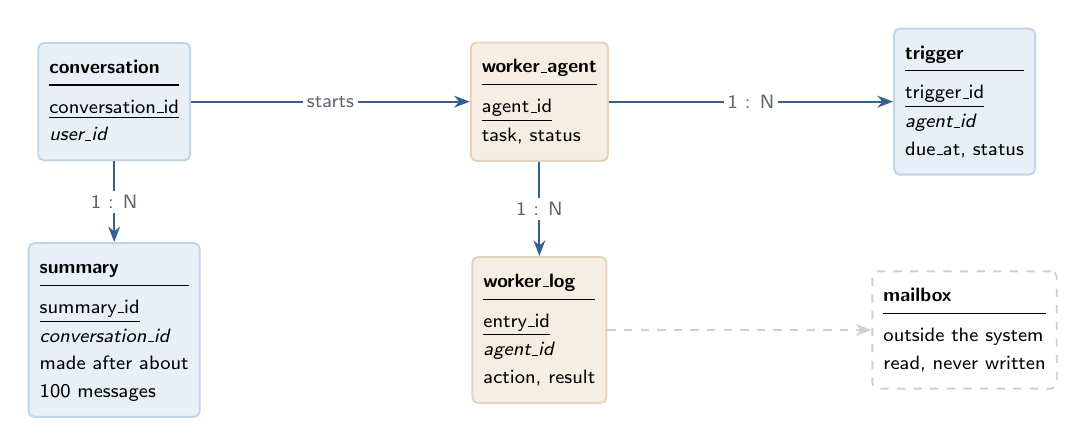
\begin{tikzpicture}
\node[ent] (conv) at (0,1.5)
  {\erE{conversation}{\pk{conversation\_id}\\ \fk{user\_id}}};
\node[ent] (summ) at (0,-1.4)
  {\erE{summary}{\pk{summary\_id}\\ \fk{conversation\_id}\\
    \scriptsize made after about\\ \scriptsize 100 messages}};
\node[entc] (work) at (5.4,1.5)
  {\erE{worker\_agent}{\pk{agent\_id}\\ task, status}};
\node[entc] (log) at (5.4,-1.4)
  {\erE{worker\_log}{\pk{entry\_id}\\ \fk{agent\_id}\\ action, result}};
\node[ent] (trig) at (10.8,1.5)
  {\erE{trigger}{\pk{trigger\_id}\\ \fk{agent\_id}\\ due\_at, status}};
\node[entn] (mail) at (10.8,-1.4)
  {\erE{mailbox}{\scriptsize outside the system\\ \scriptsize read, never written}};

\draw[ar] (conv) -- node[card,pos=0.5]{1 : N} (summ);
\draw[ar] (conv) -- node[card,pos=0.5]{starts} (work);
\draw[ar] (work) -- node[card,pos=0.5]{1 : N} (log);
\draw[ar] (work) -- node[card,pos=0.5]{1 : N} (trig);
\draw[arn] (log) -- (mail);
\end{tikzpicture}}
\caption[Poke]{Poke. Each worker owns its own log, so two workers never write
to one place. \erlegend}
\label{fig:er-poke}
\end{figure}

Poke keeps its reminders in a SQL table and checks that table once a
minute \cite{shlokedPoke}. A worker may change only its own reminders. A
poll every minute is slower than a timer, but it restarts cleanly after a
crash, and a simple query expresses it.

\textbf{Code Storage, and Git as a database.} The Pierre Computer Company
sells Git storage for machines. It offers commits, branches, and merges
through an API, and it adds short-lived branches and writes that need no
local copy \cite{codestorage,codestorageDocs}. Git belongs in this paper
because Git is a database. Table~\ref{tab:git} translates it.

\begin{table}[H]
\centering
\caption[Git parts as database parts]{Git parts, read as database parts.}
\label{tab:git}
{\small
\begin{tabularx}{\textwidth}{L{3.4cm} X}
\toprule
\sffamily\bfseries Git & \sffamily\bfseries Database \\
\midrule
Object store & Content-addressed rows. Two identical files share one row
automatically. \\
Commit & One complete version of the data, with a pointer to the version
before it. \\
Branch & A snapshot that one writer works on alone. \\
Branch update & A compare-and-swap. This is why a push fails instead of
overwriting. \\
Merge & The step that settles two changes. A plain database can only
reject one of them. \\
Reflog & The write-ahead log and the audit trail. \\
\bottomrule
\end{tabularx}}
\end{table}

The merge row matters most. When two agents change the same thing, a
key-value store keeps the last write and loses the other one. A
relational database stops one of the two transactions. Git merges them,
and it asks a person only when it cannot. Agent memory needs that third
answer, because two agents are often both right.

\emph{The next paragraph is my own design, not a description of a
product.} No public source says that Poke uses Code Storage. I pair them
because Poke's per-task workers and Code Storage's short-lived branches
fit together. Give each worker its own branch. Starting the branch is the
start of a transaction. Each commit is a private write. Merging the
branch is the commit, and the branch update fails if the main line moved,
which is exactly an optimistic retry. Dropping an abandoned branch costs
nothing.

%=====================================================================
\section{Comparison}
%=====================================================================

\begin{table}[H]
\centering
\caption[How the four systems carry memory]{How the four systems carry memory across a session boundary.}
\label{tab:cmp}
{\footnotesize
\renewcommand{\arraystretch}{1.3}
\begin{tabularx}{\textwidth}{L{1.8cm} X X}
\toprule
\sffamily\bfseries System & \sffamily\bfseries What crosses the boundary &
\sffamily\bfseries The idea worth copying \\
\midrule
OpenClaw & Markdown files, with a SQLite index built from them &
Keep the original readable and treat the index as a copy \\
Hermes & One SQLite file of every message, plus two size-limited notes &
Set a quota and fail the write, instead of cleaning up later \\
eve and Benji & Step checkpoints in a durable store, plus Benji's two
levels of notes & Give each helper its own state, so no two can collide \\
Poke and Code Storage & A private log for each worker, plus reminders in
a SQL table & Use a merge to settle a conflict, not a rejection \\
\bottomrule
\end{tabularx}}
\end{table}

\subsection{What the four systems agree on}

\textbf{They all use more than one store.} Every system keeps small
facts apart from large history. The two have different sizes and
different read patterns, so one engine cannot serve both well.

\textbf{They all keep files.} Three of the four keep the curated facts in
readable files and use the database as the index. A person can open a
file, read what the agent believes, and correct it. This matters more
than it first appears.

\textbf{They all search twice.} No system searches by meaning alone.
Vectors miss file names, error strings, and version numbers, so a text
search always runs beside the vector search.

\textbf{They all set limits.} Hermes sets a token quota. OpenClaw returns
six rows. Benji needs three repositories. A store that grows without a
limit gets slower and less accurate at the same time.

\textbf{They avoid sharing instead of locking.} None of the four uses a
strict isolation level to coordinate writers. eve gives each helper its
own state. Poke gives each worker its own log. Git gives each agent its
own branch. They remove the shared cell rather than guard it. This works
until the agents must share what they learned, which is exactly Benji's
promotion step.

\textbf{They all skip validity periods.} No system in this study records
when a fact stops being true. Databases solved this problem long ago.
Agents have not adopted it yet.

%=====================================================================
\section{Design Rules}
%=====================================================================

\begin{enumerate}
  \item \textbf{Keep the log as the original.} Build every index from it.
        A wrong index then costs a rebuild, not the data.
  \item \textbf{Return few rows.} Six correct rows beat fifty correct
        rows, because the prompt is the scarce resource.
  \item \textbf{Set a quota and fail the write.} The agent then sees the
        limit and merges its notes itself.
  \item \textbf{Give each helper its own state.} Add a constraint only at
        the few points where helpers must share.
  \item \textbf{Put the safety rule in the schema.} A constraint holds
        even when the program is wrong.
  \item \textbf{Give every fact a period.} Close the old period, open a
        new one, and never overwrite.
  \item \textbf{Keep the memory readable.} A person must be able to open
        it and correct it.
\end{enumerate}

%=====================================================================
\section{Limits of This Study}
%=====================================================================

I ran no experiments. The schema and the queries compile, but I did not
measure them against a workload, so every performance statement here is
reasoning and not a result. I read public documents and public source, so
the descriptions can lag the code. Poke is closed software, and I built
that section from a third-party write-up \cite{shlokedPoke}. All four
projects change quickly, so a reader should check the current documents
before relying on a table name or a setting. I chose the four systems
because they are well documented and different from each other, not by
any sampling rule.

%=====================================================================
\section{Conclusion}
%=====================================================================

An agent's memory is not part of the model. It is a database, and the
agent behaves well over weeks only when that database is well designed.

The four layers in this paper separate a log that never changes from
tables that carry constraints, an index that the team can rebuild, and a
prompt that the system discards after every call. Each separation follows
from a difference in access pattern or in the cost of a loss. The schema
that results is ordinary. It normalises to Boyce--Codd normal form, it
takes ordinary indexes, and one SQL statement expresses the recall.

The four systems resolve the same tensions in four defensible ways.
OpenClaw shows that a readable original plus a rebuildable index is a
strong pairing. Hermes shows that a hard quota produces a more
predictable agent than unlimited growth. eve shows that a framework
should refuse to widen the scope of its state, and Benji shows that a
counting rule stops one project's habit from spreading. Poke shows that
one log per worker removes a whole class of concurrency fault, and Code
Storage shows that Git already offers the merge that relational memory
lacks.

Two gaps remain. No system records when a fact stops being true. No
agreed method exists for two agents that must write to one memory, only
the practice of avoiding shared state. Both gaps have answers in the
database literature. The field would move faster if it read them.

%=====================================================================
\begin{thebibliography}{99}
\addcontentsline{toc}{section}{References}
{\small\setlength{\itemsep}{0.35\baselineskip}

\bibitem{codd1970} E. F. Codd. ``A Relational Model of Data for Large
Shared Data Banks.'' \emph{Communications of the ACM}, 13(6):377--387,
1970.

\bibitem{harder1983} T. Härder and A. Reuter. ``Principles of
Transaction-Oriented Database Recovery.'' \emph{ACM Computing Surveys},
15(4):287--317, 1983.

\bibitem{berenson1995} H. Berenson, P. Bernstein, J. Gray, J. Melton,
E. O'Neil and P. O'Neil. ``A Critique of ANSI SQL Isolation Levels.''
\emph{Proceedings of ACM SIGMOD}, 1995.

\bibitem{fekete2005} A. Fekete, D. Liarokapis, E. O'Neil, P. O'Neil and
D. Shasha. ``Making Snapshot Isolation Serializable.'' \emph{ACM
Transactions on Database Systems}, 30(2):492--528, 2005.

\bibitem{snodgrass2000} R. T. Snodgrass. \emph{Developing Time-Oriented
Database Applications in SQL}. Morgan Kaufmann, 2000.

\bibitem{kleppmann2017} M. Kleppmann. \emph{Designing Data-Intensive
Applications}. O'Reilly Media, 2017.

\bibitem{malkov2018} Y. A. Malkov and D. A. Yashunin. ``Efficient and
Robust Approximate Nearest Neighbor Search Using Hierarchical Navigable
Small World Graphs.'' \emph{IEEE TPAMI}, 42(4):824--836, 2020.

\bibitem{lewis2020} P. Lewis et al. ``Retrieval-Augmented Generation for
Knowledge-Intensive NLP Tasks.'' \emph{NeurIPS}, 2020.

\bibitem{park2023} J. S. Park, J. C. O'Brien, C. J. Cai, M. R. Morris,
P. Liang and M. S. Bernstein. ``Generative Agents: Interactive Simulacra
of Human Behavior.'' \emph{Proceedings of ACM UIST}, 2023.

\bibitem{packer2023} C. Packer et al. ``MemGPT: Towards LLMs as
Operating Systems.'' arXiv:2310.08560, 2023.

\bibitem{gruber2026} J. Gruber and J.-N. Hilgert. ``Foundations for
Agentic AI Investigations from the Forensic Analysis of OpenClaw.''
arXiv:2604.05589, 2026. \url{https://arxiv.org/abs/2604.05589}

\bibitem{openclawRepo} OpenClaw Foundation. ``OpenClaw.'' GitHub.
\url{https://github.com/openclaw/openclaw}

\bibitem{openclawMemCfg} OpenClaw. ``Memory Configuration Reference.''
\url{https://docs.openclaw.ai/reference/memory-config}

\bibitem{tcOpenClaw} \emph{TechCrunch}. ``OpenClaw Creator Peter
Steinberger Joins OpenAI.'' 15 February 2026.
\url{https://techcrunch.com/2026/02/15/openclaw-creator-peter-steinberger-joins-openai/}

\bibitem{forbesOpenClaw} R. Schmelzer. ``OpenAI Hires OpenClaw Creator
Peter Steinberger And Sets Up Foundation.'' \emph{Forbes}, 16 February
2026.
\url{https://www.forbes.com/sites/ronschmelzer/2026/02/16/openai-hires-openclaw-creator-peter-steinberger-and-sets-up-foundation/}

\bibitem{hermesRepo} Nous Research. ``Hermes Agent.'' GitHub.
\url{https://github.com/NousResearch/hermes-agent}

\bibitem{hermesArch} Nous Research. ``Architecture.'' Hermes Agent
Developer Guide.
\url{https://hermes-agent.nousresearch.com/docs/developer-guide/architecture}

\bibitem{hermesMemory} Nous Research. ``Persistent Memory.'' Hermes Agent
User Guide.
\url{https://hermes-agent.nousresearch.com/docs/user-guide/features/memory/}

\bibitem{hermesDeepwiki} ``Memory and Sessions --- NousResearch/hermes-agent.''
DeepWiki.
\url{https://deepwiki.com/NousResearch/hermes-agent/4.3-memory-and-sessions}

\bibitem{eveSite} Vercel. ``eve --- The Framework for Building Agents.''
\url{https://eve.dev/}

\bibitem{eveDurability} Vercel. ``Execution Model and Durability.'' eve
Documentation.
\url{https://eve.dev/docs/concepts/execution-model-and-durability}

\bibitem{eveState} Vercel. ``State.'' eve Documentation.
\url{https://eve.dev/docs/guides/state}

\bibitem{benjiRepo} AgentsORG. ``Benji.'' GitHub.
\url{https://github.com/AgentsORG/Benji}

\bibitem{agentsorg} AgentsORG. \url{https://agents.org.in}

\bibitem{shlokedPoke} S. Khemani. ``OpenPoke: Recreating Poke's
Architecture.'' \url{https://www.shloked.com/writing/openpoke}

\bibitem{tcPoke} \emph{TechCrunch}. ``Why Cognition Bought Poke.''
24 July 2026.
\url{https://techcrunch.com/2026/07/24/why-cognition-bought-poke-ai-personality-is-becoming-a-competitive-advantage/}

\bibitem{codestorage} The Pierre Computer Company. ``Code Storage.''
\url{https://code.storage/}

\bibitem{codestorageDocs} The Pierre Computer Company. ``Code Storage
Documentation.'' \url{https://code.storage/docs}

\bibitem{pierreCo} The Pierre Computer Company.
\url{https://pierre.computer/}

\bibitem{sqliteWal} SQLite Consortium. ``Write-Ahead Logging.''
\url{https://www.sqlite.org/wal.html}

\bibitem{sqliteFts5} SQLite Consortium. ``FTS5 Extension.''
\url{https://www.sqlite.org/fts5.html}

\bibitem{pgvector} A. Kane. ``pgvector.'' GitHub.
\url{https://github.com/pgvector/pgvector}
}
\end{thebibliography}

\vspace{1.2\baselineskip}
{\color{blue200}\rule{\textwidth}{0.5pt}}\\[5pt]
{\footnotesize\sffamily\color{grey600}
\khe\ \quad\textperiodcentered\quad 241302081 \quad\textperiodcentered\quad
B.Tech CSE (AI/ML), Section C\\[2pt]
Department of Computer Science \& Engineering, SGT University}

\end{document}
